\documentclass{article}
\usepackage[utf8]{inputenc}
\textheight = 25cm 
\textwidth = 15cm
\topmargin = -3.0cm 
\oddsidemargin = 1.5cm
\usepackage{hyperref}
\hypersetup{
    colorlinks=true,
    linkcolor=blue,
    filecolor=blue,
    citecolor=black,      
    urlcolor=blue,
    }

\usepackage{float}
\usepackage{graphicx}

\usepackage{gensymb}

\usepackage{amsmath}
\usepackage{amssymb}
\usepackage{amsfonts}
\usepackage{mathtools, xparse}
\usepackage[shortlabels]{enumitem}

\usepackage[many]{tcolorbox}
\usepackage{lipsum}
\usepackage{amssymb}

\title{Cuestionario 1 Termodinámica}
\author{Cerritos Lira, Carlos}
\date{18 de Mayo del 2020}

\newcommand{\pr}[1]{\left(#1\right)}
\newcommand{\pt}[2]{\dfrac{\partial #1}{\partial #2}}

\begin{document}
\maketitle
\section*{1.-}
¿Cuáles son las diferencias que permitieron mejorar la eficiencia de la máquina de Watt en 
comparación con la de Newcomen?
\begin{tcolorbox}[breakable]
    El motor de Newcomen usa la presión del vació que se genera después de la condensación 
    de agua dentro de un cilindro. Fue usado para sacar agua de las minas. \\
    Watt invento un enfriador o condensador separado, al cual entraba el vapor una vez se abría 
    una válvula, entre otras mejoras como:
    \begin{enumerate}
        \item Mantener caliente la pared del cilindro (debido a que la condensación no ocurría en esté).
        \item Hacer funcionar el pistón tanto en la carrera descendene como en la ascendente.
        \item Cerrar la válvula de vapor antes del final de la carrera.
    \end{enumerate}
    \end{tcolorbox}

\section*{2.-}
¿Por qué se dice que el motor de watt era más que una bomba?
\begin{tcolorbox}[breakable]
    La máquina de Watt tranformo el movimiento lineal en circular (la rotación de una rueda),
    debido a esto pudo usarse en tareas mas diversas, como por ejemplo: tornos, taladros, 
    ruedas giratorias, telares, barcos y locomotoras.
    \begin{figure}[H]
        \centering
        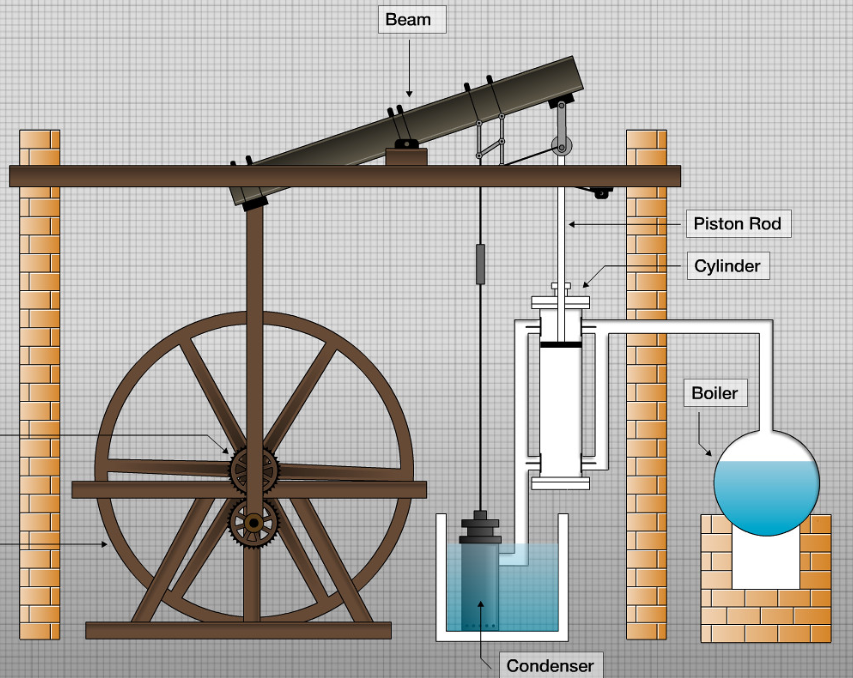
\includegraphics[scale=0.35]{images/p2_watt.png}
        \caption{Máquina de Watt}
        \label{}
    \end{figure}
\end{tcolorbox}

\section*{3.-}
Del libro de Martínez Negrete páginas $170-178$ mencione las analogías entre el motor hidráulico
(Lázaro Carnot) y el motor de Carnot(Sadi Carnot), explicando:
\begin{enumerate}
    \item Relación agua-calor 
    \item Relación altura-temperatura
\end{enumerate}
\begin{tcolorbox}[breakable]
    De acuerdo a la analogía de Sadi Carnot, el motor térmico y el motor hidráulico comparten ciertas 
    características.
    \textit{Se puede comparar con bastante exactitud la potencia motriz del calor con la de un salto de agua.}
    \subsubsection*{Relación altura-temperatura}
    El calórico es un fluido hipotético que va de los cuerpos calientes a los fríos, ánalogo al agua.
    \subsubsection*{Relación agua-calórico}
    Así como una rueda hidráulica necesita una diferencia de altura, lo mismo debe ocurrir para el motor 
    térmico, debe existir una diferencia de temperatura para el calórico. 
\end{tcolorbox}

\section*{4.-}
Del mismo texto describa el ciclo de operación reversible en el motor de agua y su semejante con el motor térmico.
\begin{tcolorbox}[breakable]
    \begin{itemize}
        \item Se recibe una cantidad de agua de masa $m$ a la altura $h_1$ a una velocidad relativa cercana a $0$.
        \item La masa de agua baja lentamente sin pérdida, hasta llegar a una altura $h_2$.
        \item La rueda abandona el cangilón a velocidad relativa cercana a $0$.
        \item El cangilón vació llega de nuevo a la altura $h_1$, y el ciclo se repite.
    \end{itemize}
    Estos 4 procesos son análogos a los del ciclo de un motor térmico:
    \begin{itemize}
        \item Energetización por calor $Q_1$ de la sustancia con la que se trabaja (vapor de agua).
        \item Se realiza una expansión adiabática hasta llegar a la temperatura $T_2$
        \item El vapor se comprime isotérmicamente a $T_2$ 
        \item Se realiza una compresión adiabática hasta elevar la temperatura a $T_1$, y el ciclo se repite.   
    \end{itemize}
\end{tcolorbox}

\section*{5.-}
¿Qué aspecto fundamental descubre Carnot sobre las sustancias de trabajo de su motor?
\begin{tcolorbox}[breakable]
    Carnot descubrio que la eficiencia solo dependia de la diferencia de temperatura de los focos y no de la sustancia, 
    además de esto diseño el motor de Carnot, el cuál tiene la eficiencia más alta que se puede conseguir, donde:
    \[ \rho_{max} = 1 - \frac{T_C}{T_H} \]
\end{tcolorbox}

\section*{6.-}
¿Cuál es la relación entre un móvil perpetuo y una máquina que trabaja con un solo foco témico?
\begin{tcolorbox}[breakable]
    Un móvil perpetuo de segunda especie es una máquina que espontanemente convierte energía térmica en trabajo mecánico con eficiencia 1. \\
    Al tener una máquina que trabaja con un solo foco térmico tendríamos una eficiencia de 1 lo que la convertiria en un móvil perpetu de segunda especie.
\end{tcolorbox}


\end{document}